\chapter{Reti sequenziali}

\section{Cosa è un circuito (o rete) sequenziale?}
Un circuito (o rete) sequenziale è un circuito in cui lo stato delle uscite non dipende solo dalla funzione logica applicata ai suoi ingressi, ma anche sulla base di valori pregressi collocati in memoria

\section{Componenti}
I circuiti sequenziali sono formati da:
\begin{itemize}
    \item Elementi di memoria (di vario tipo): Memorizzano l'informazione
    \item Reti combinatorie: Elaborano l'informazione
\end{itemize}

\section{Stato}
Un circuito sequenziale ha, in ogni dato istante, uno stato determinato dai bit memorizzati

\begin{center}
\begin{tikzpicture}[
    font=\sffamily,
    >=stealth,
    box/.style={draw, minimum width=3.5cm, minimum height=1.8cm, align=center},
    node distance=2.5cm
]

    % Definizione dei due blocchi principali
    \node[box] (mem) {Elementi \\ di memoria};
    \node[box, right=2cm of mem, yshift=1cm] (comb) {Circuito \\ combinatorio};

    % Ingressi
    % Creiamo una coordinata fittizia a sinistra per far partire la freccia degli Ingressi
    \coordinate (in_start) at ([xshift=-4.5cm]comb.165);
    \draw[->] (in_start) node[left] {Ingressi} -- (comb.165);

    % Uscite
    \draw[->] (comb.15) -- ++(1.5,0) node[right] {Uscite};

    % Stato Corrente (da mem a comb)
    \draw[->] (mem.east) -- (comb.195) node[midway, align=left, above] {Stato \\ corrente};

    % Stato Successivo (feedback da comb a mem)
    % Usiamo percorsi ortogonali (|- e -|) per fare il loop rettangolare verso il basso
    \draw[->] (comb.345) -- ++(1,0) |- ([yshift=-1cm]mem.south) -| ([xshift=-1cm]mem.west) -- (mem.west) 
        node[pos=0.15, above] {Stato successivo};

\end{tikzpicture}
\end{center}

\section{Famiglie di circuiti sequenziali}
Esistono 2 famiglie di circuiti digitali sequenziali:
\begin{itemize}
    \item \textbf{Asincroni}: Non fanno uso del clock
    \item \textbf{Sincroni}: Necessitano dell'utilizzo del clock
\end{itemize}

\newpage
\section{Clock}
\subsection{Cosa è?}
È un segnale (onda quadra) con periodo predeterminato e costante

\subsection{Diagramma}
\begin{center}
    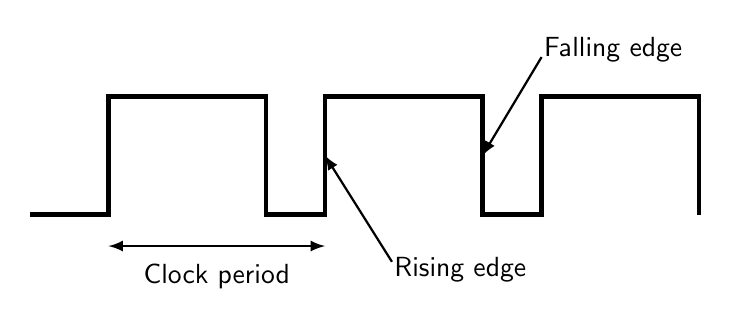
\begin{tikzpicture}[font=\sffamily, >=latex, thick]

        % ==========================================
        % 1. Segnale di Clock (Onda quadra)
        % ==========================================
        \draw[line width=1.5pt] 
            (0,0) -- (1,0) -- (1,1.5) -- (3,1.5) -- (3,0) -- 
            (3.75,0) -- (3.75,1.5) -- (5.75,1.5) -- (5.75,0) -- 
            (6.5,0) -- (6.5,1.5) -- (8.5,1.5) -- (8.5,0);

        % ==========================================
        % 2. Indicatore del Periodo (Clock period)
        % ==========================================
        \draw[<->, line width=0.8pt] (1, -0.4) -- (3.75, -0.4);
        \node[below] at (2.375, -0.5) {Clock period};

        % ==========================================
        % 3. Indicatore Fronte di Salita (Rising edge)
        % ==========================================
        \draw[<-, line width=0.8pt] (3.75, 0.75) -- (4.6, -0.6);
        \node[right] at (4.5, -0.7) {Rising edge};

        % ==========================================
        % 4. Indicatore Fronte di Discesa (Falling edge)
        % ==========================================
        \draw[<-, line width=0.8pt] (5.75, 0.75) -- (6.5, 2.0);
        \node[right] at (6.4, 2.1) {Falling edge};

    \end{tikzpicture}
\end{center}

\subsection{Formula: Frequenza di clock}
\begin{center}
    \begin{tcolorbox}[title=Frequenza di clock,width=0.65\textwidth]
        {
            \Large
            $$
            F = \frac{1}{T}
            $$

            \begin{itemize}
                \item $T$ = Periodo / ciclo di clock
                \item $F$ = Frequenza di clock
            \end{itemize}
        }
    \end{tcolorbox}
\end{center}

\newpage
\section{S-R Latch}
\subsection{Cosa è?}
È un circuito composto da 2 porte NOR concatenate

\begin{minipage}{0.50\textwidth}
    \subsection{Schema}
    \begin{center}
        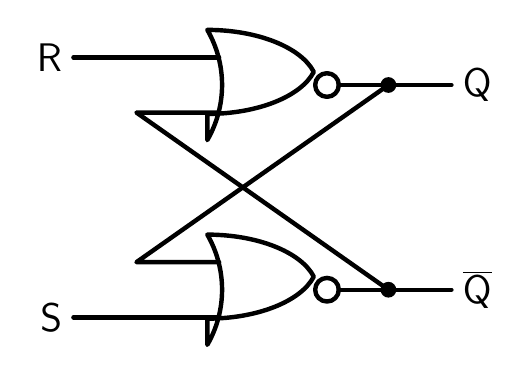
\begin{tikzpicture}[font=\Large\sffamily, line width=1.6pt, line cap=round, line join=round]

            % ==========================================
            % 1. Porta NOR Superiore
            % ==========================================
            \begin{scope}[shift={(0, 1.3)}]
                \draw (-0.1, -0.7) 
                    arc[start angle=-30, end angle=30, radius=1.4] 
                    arc[start angle=90, end angle=15, x radius=1.4, y radius=0.72]
                    arc[start angle=-15, end angle=-90, x radius=1.4, y radius=0.72] 
                    -- cycle;
                \draw (1.42, 0) circle (0.15);
                \draw (1.57, 0) -- (3.0, 0) node[right] {Q};
            \end{scope}

            % ==========================================
            % 2. Porta NOR Inferiore
            % ==========================================
            \begin{scope}[shift={(0, -1.3)}]
                \draw (-0.1, -0.7) 
                    arc[start angle=-30, end angle=30, radius=1.4] 
                    arc[start angle=90, end angle=15, x radius=1.4, y radius=0.72]
                    arc[start angle=-15, end angle=-90, x radius=1.4, y radius=0.72] 
                    -- cycle;
                \draw (1.42, 0) circle (0.15);
                \draw (1.57, 0) -- (3.0, 0) node[right] {$\overline{\mathsf{Q}}$};
            \end{scope}

            % ==========================================
            % 3. Ingressi Esterni (R e S)
            % ==========================================
            \draw (-1.8, 1.65) node[left] {R} -- (0.05, 1.65);
            \draw (-1.8, -1.65) node[left] {S} -- (0.05, -1.65);

            % ==========================================
            % 4. Cablaggio incrociato (Cross-Coupled Feedback)
            % ==========================================
            \fill (2.2, 1.3) circle (0.1);
            \fill (2.2, -1.3) circle (0.1);

            \draw (2.2, 1.3) -- (-1.0, -0.95) -- (0.05, -0.95);
            \draw (2.2, -1.3) -- (-1.0, 0.95) -- (0.05, 0.95);

        \end{tikzpicture}
    \end{center}
\end{minipage}
\hfil
\begin{minipage}{0.15\textwidth}
    \begin{center}
        {
            \Large
            S = Set

            R = Reset
        }
    \end{center}
\end{minipage}

\subsection{Tabella}
\begin{minipage}[t]{0.35\textwidth}
    \begin{center}
        \begin{tabular}{|c|c|c|c|c|}
            \hline
            \multicolumn{2}{|c|}{Input} & Stato Interno & \multicolumn{2}{c|}{Output} \\
            \multicolumn{1}{|c}{S} & \multicolumn{1}{c|}{R} & Old Q & \multicolumn{1}{c}{Q} & \multicolumn{1}{c|}{$\overline{\mathsf{Q}}$} \\
            \hline
            0 & 0 & 0 & 0 & 1 \\
            \hline
            0 & 0 & 1 & 1 & 0 \\
            \hline
            0 & 1 & 1/0 & 0 & 1 \\
            \hline
            1 & 0 & 1/0 & 1 & 0 \\
            \hline
            1 & 1 & 1/0 & 0 & 0 \\
            \hline
        \end{tabular}
    \end{center}
\end{minipage}
\hfil
\begin{minipage}{0.6\textwidth}
    \begin{itemize}
        \item La combinazione (S,R) = (0,0) viene detta combinazione di riposo, perchè semplicemente mantiente il valore memorizzato in precedenza
        
        \vspace{0.3cm}

        \item La combinazione (S,R) = (1,1) viola la proprietà di complementarietà di $Q$ e $\overline{Q}$, può portare ad una configurazione instabile
    \end{itemize}
\end{minipage}

\subsection{Problematiche}
In un SR Latch il valore di Q all'accensione dell'elaboratore è indeterminato, a meno che non ci sia un meccanismo di inizializzazione

\begin{itemize}
    \item All'accensione, i valori interni dei nodi dipendono da condizioni casuali, come la carica residua nei transisto o nei condensatori
    \item Se non viene forzato un valore iniziale, il latch potrebbe assumere un qualsiasi stato in modo casuale.
    \begin{itemize}
        \item \textbf{Reset Hardware}: Un segnale di reset globale può forzare $Q=0$ e $\overline{Q}=1$ subito dopo l'accensione
        \item \textbf{SR con Priorità di Reset}: Se il circuito include un reset attivo all'avvio, $Q$ sarà forzato a un valore noto
    \end{itemize}
\end{itemize}

\newpage
\section{D Latch}
\subsection{Definizione}
È un Latch sincronizzato con il clock, la sincronizzazione con il clock garantisce che il latch cambi stato solo in certi momenti

\subsection{Schema}
\begin{minipage}{0.4\textwidth}
    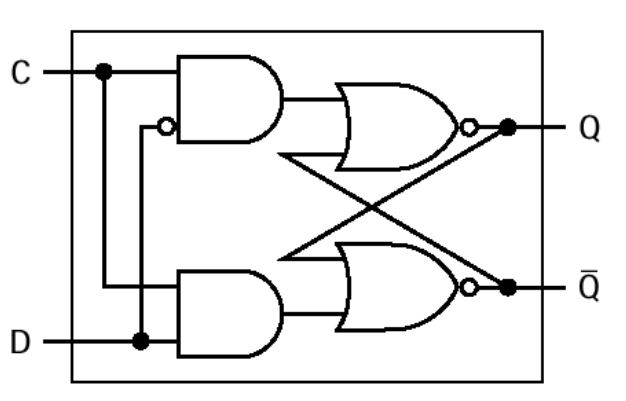
\includegraphics[scale=0.4]{Immagini/D-Latch.png}
\end{minipage}
\hfil
\begin{minipage}{0.45\textwidth}
    {
        \large

        \begin{itemize}
            \item $\mathbf{D=1}$ corrisponde al setting
            \begin{itemize}
                \item $S=1$ e $R=0$
            \end{itemize}
            \item $\mathbf{D=0}$ corrisponde al resetting
            \begin{itemize}
                \item $S=0$ e $R=1$
            \end{itemize}
        \end{itemize}
    }
\end{minipage}

\begin{center}
    \begin{itemize}
    \item Quando \textbf{il clock è deasserted} non viene memorizzato nessun valore:
    \begin{itemize}
        \item $S=0$ e $R=0$ (viene mantenuto il valore precedentemente memorizzato)
    \end{itemize}

    \item  Quando \textbf{il clock è asserted} viene memorizzato un valore (in funzione del valore di $D$)
    \end{itemize}
\end{center}

\subsection{Comportamento}
Il D-Latch è caratterizzato dal seguente comportamento:
\begin{enumerate}
    \item Durante l'intervallo alto del clock il valore del segnale di ingresso D viene memorizzato nel latch
    \item Il valore D si propaga quasi immediatamente all'uscita Q
    \item Anche le eventuali variazioni di D si propagano quasi immediatamente, con il risultato che Q può variare più volte durante l'intervallo alto del clock
    \item Solo quando il clock torno a zero Q si stabilizza
    \item Durante l'intervallo basso del clock il latch non memorizza
\end{enumerate}

\subsection{Segnale $D$}
Il segnale D ottenuto come output di un circuito combinatorio deve:
\begin{itemize}
    \item Essere già stabile quando $C$ diventa asserted
    \item Rimanere stabile per tutta la durata del livello alto di $C$ (Setup time)
    \item Rimanere stabile per un altro periodo di tempo per evitare malfunzionamenti (Hold time)
\end{itemize}

\begin{center}
    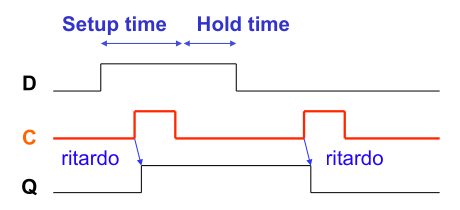
\includegraphics[scale=0.5]{Immagini/Segnale T.png}
\end{center}

\subsection{Lunghezza periodo di clock $T$}
Il periodo di clock $T$ deve essere scelto abbastanza lungo affinchè l'output del circuito combinatorio si stabilizzi

\begin{center}
    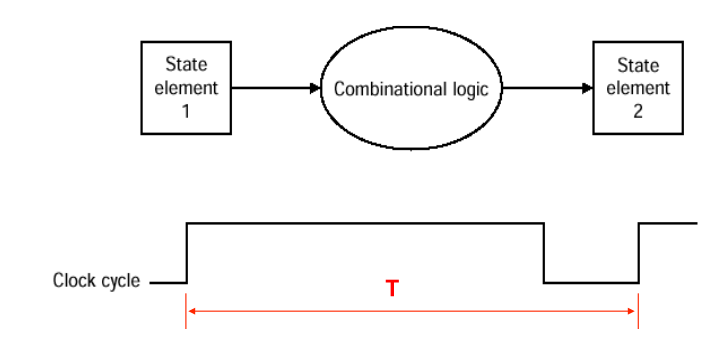
\includegraphics[scale=0.5]{Immagini/Lunghezza clock T.png}
\end{center}

\newpage
\section{D Flip-Flop}
\subsection{Metodologie di timing}
Fino ad ora abbiamo visto  una metodologia di timing detta \textbf{level-triggered} che avviene sul livello alto (o basso del clock)

Esiste una metodologia di timing chiamata \textbf{edge-triggered} che avviene sul fronte di salita (o di discesa) del clock
\begin{itemize}
    \item La memorizzazione avviene istantaneamente
    \item L'eventuale segnale di ritorno "sporco" non fa in tempo ad arrivare a causa dell'istantaneata della memorizzazione
\end{itemize}

\subsection{Definizione}
Il D Flip-Flop è usabile come input e output durante lo stesso ciclo di clock, viene realizzato ponendo in serie 2 D-Latch: il primo viene detto \textbf{master} e il secondo \textbf{slave}


\begin{minipage}[t]{0.45\textwidth}
    \subsection{Schema}
        \begin{center}
            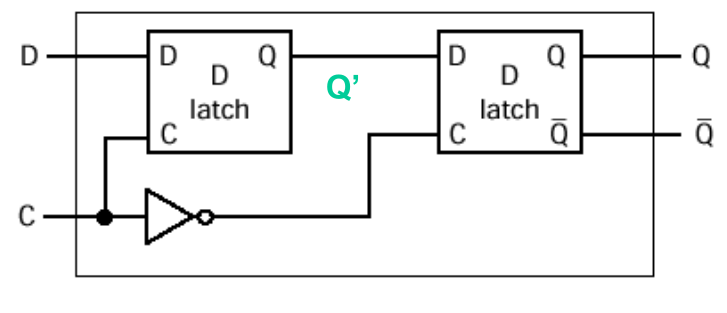
\includegraphics[scale=0.35]{Immagini/D FlipFlop Schema.png}
        \end{center}
    \subsection{Schema dei segnali}
        \begin{center}
            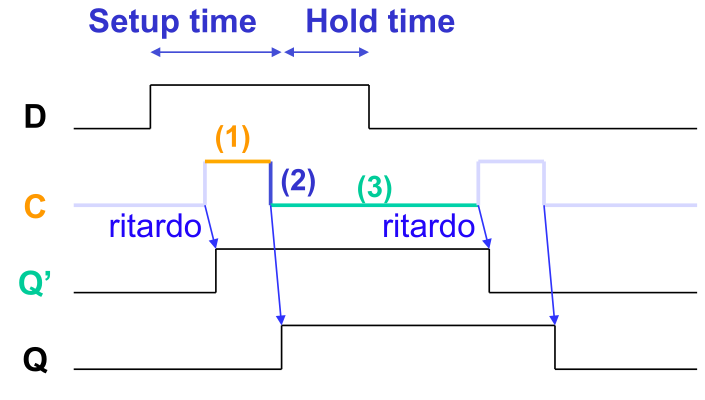
\includegraphics[scale=0.35]{Immagini/D FlipFlop Segnale.png}
        \end{center}
\end{minipage}
\hfil
\begin{minipage}[t]{0.45\textwidth}
    \subsection{Funzionamento}
        \begin{enumerate}
            \item Il primo latch è aperto e pronto per memorizzare D. \\
            Il valore memorizzato Q fluisce fuori, ma il secondo latch è chiuso 
            \begin{itemize}
                \item Nel circuito combinatorio a valle entra ancora il vecchio valore di Q
            \end{itemize}

            \item Il segnale del clock scende, e in questo istante il secondo latch viene aperto per memorizzare il valore di Q
            
            \item Il secondo latch è aperto, memorizza D, e fa fluire il nuovo valore Q nel circuito a valle.\\
            Il primo latch p invece chiuso, e non memorizza niente
        \end{enumerate}
\end{minipage}
